\documentclass{beamer}
\mode<presentation>
\usepackage{amsmath}
\usepackage{amssymb}
%\usepackage{advdate}
\usepackage{adjustbox}
\usepackage{subcaption}
\usepackage{enumitem}
\usepackage{multicol}
\usepackage{listings}
\usepackage{url}
\def\UrlBreaks{\do\/\do-}
\usetheme{Boadilla}
\usecolortheme{lily}
\setbeamertemplate{footline}
{
  \leavevmode%
  \hbox{%
  \begin{beamercolorbox}[wd=\paperwidth,ht=2.25ex,dp=1ex,right]{author in head/foot}%
    \insertframenumber{} / \inserttotalframenumber\hspace*{2ex} 
  \end{beamercolorbox}}%
  \vskip0pt%
}
\setbeamertemplate{navigation symbols}{}

\providecommand{\nCr}[2]{\,^{#1}C_{#2}} % nCr
\providecommand{\nPr}[2]{\,^{#1}P_{#2}} % nPr
\providecommand{\mbf}{\mathbf}
\providecommand{\pr}[1]{\ensuremath{\Pr\left(#1\right)}}
\providecommand{\qfunc}[1]{\ensuremath{Q\left(#1\right)}}
\providecommand{\sbrak}[1]{\ensuremath{{}\left[#1\right]}}
\providecommand{\lsbrak}[1]{\ensuremath{{}\left[#1\right.}}
\providecommand{\rsbrak}[1]{\ensuremath{{}\left.#1\right]}}
\providecommand{\brak}[1]{\ensuremath{\left(#1\right)}}
\providecommand{\lbrak}[1]{\ensuremath{\left(#1\right.}}
\providecommand{\rbrak}[1]{\ensuremath{\left.#1\right)}}
\providecommand{\cbrak}[1]{\ensuremath{\left\{#1\right\}}}
\providecommand{\lcbrak}[1]{\ensuremath{\left\{#1\right.}}
\providecommand{\rcbrak}[1]{\ensuremath{\left.#1\right\}}}
\theoremstyle{remark}
\newtheorem{rem}{Remark}
\newcommand{\sgn}{\mathop{\mathrm{sgn}}}
\providecommand{\abs}[1]{\left\vert#1\right\vert}
\providecommand{\res}[1]{\Res\displaylimits_{#1}} 
\providecommand{\norm}[1]{\lVert#1\rVert}
\providecommand{\mtx}[1]{\mathbf{#1}}
\providecommand{\mean}[1]{E\left[ #1 \right]}
\providecommand{\fourier}{\overset{\mathcal{F}}{ \rightleftharpoons}}
%\providecommand{\hilbert}{\overset{\mathcal{H}}{ \rightleftharpoons}}
\providecommand{\system}{\overset{\mathcal{H}}{ \longleftrightarrow}}
	%\newcommand{\solution}[2]{\textbf{Solution:}{#1}}
%\newcommand{\solution}{\noindent \textbf{Solution: }}
\providecommand{\dec}[2]{\ensuremath{\overset{#1}{\underset{#2}{\gtrless}}}}
\newcommand{\myvec}[1]{\ensuremath{\begin{pmatrix}#1\end{pmatrix}}}
\let\vec\mathbf

\lstset{
%language=C,
frame=single, 
breaklines=true,
columns=fullflexible
}

\numberwithin{equation}{section}

\title{12.8.ex12}
\author{Prajwal \\ EE24BTECH11051}
\begin{document}

\begin{frame}
\titlepage
\end{frame}
\section*{Outline}
\begin{frame}
\tableofcontents
\end{frame}
\section{Problem}
\begin{frame}
\frametitle{Problem Statement}
Find the area of the region bounded by the line $y=3x+2,$ the x-axis and the ordinates $x=-1$ and $x=1.$ 
\end{frame}
%\subsection{Literature}
\section{Solution}
\subsection{Theoretical Solution}
\begin{frame}
\frametitle{Theoretical Solution}
    Set up the integral: \\
    The area under the curve can be calculated as:
    \begin{align}
          \text{Area}=\int_{a}^{b}f(x)dx
    \end{align}
     Here:
    \begin{align}
    f(x) = 3x+2, \quad x_1 = -1, \quad x_2 = 1
    \end{align}
    Check whether the line touches the x-axis in the interval $x\in\brak{-1,1}$ \\
    \begin{align}
        y=0=3x+2\\
        x=\frac{-2}{3}\\
    \end{align}
    As $x=\frac{-2}{3}\in \brak{-1,1}$
\end{frame}
\begin{frame}
    Thus, the integral becomes:
    \begin{align}
    \text{Area} = -\int_{-1}^{-2/3} (3x+2)  \, dx+\int_{-2/3}^{1} (3x+2) \, dx
    \end{align}
    \item Compute the integral: \\
    The integral of $3x+2$ is:
    \begin{align}
    \int 3x+2 \, dx = \frac{3x^2}{2}+2x
    \end{align}
    \item Evaluate the definite integral: \\
    Substitute the limits of integration:
    \begin{align}
    \text{Area} = -\sbrak{\frac{3x^2}{2}+2x}_{-1}^{-2/3}+\sbrak{\frac{3x^2}{2}+2x}_{-2/3}^{1} \\
    \text{Area} = \frac{13}{3}
    \end{align}
\end{frame}
\section{Plot}
\subsection{Graph}
\begin{frame}[fragile]
\frametitle{Plot}
    \begin{figure}[htbp] % Positioning options: here, top, bottom, page
    \centering
    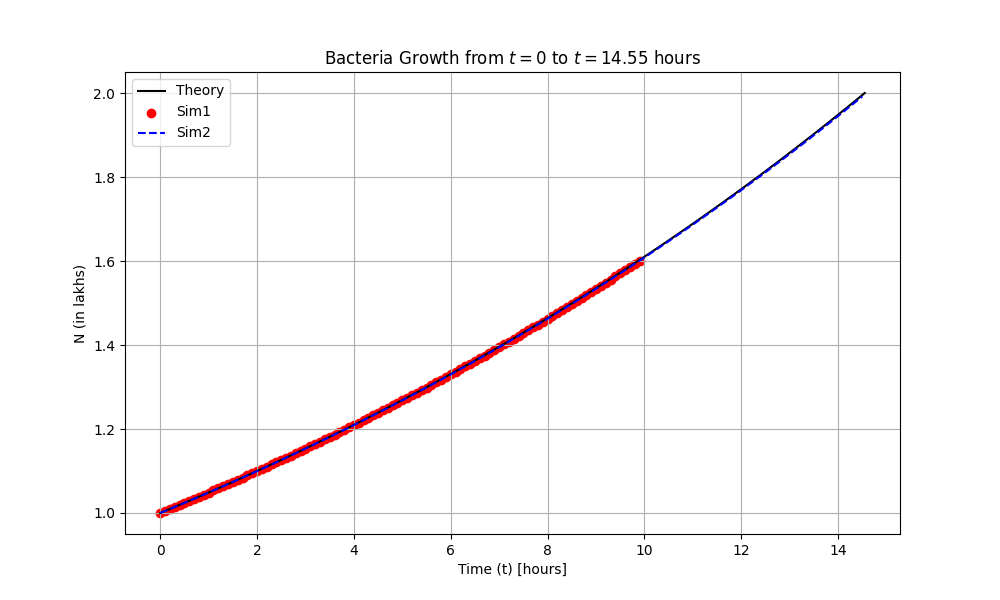
\includegraphics[width=\textwidth]{figs/plot.png} % Replace "filename" with your image file
    \caption{Number of bacteria vs time}
\end{figure}
\end{frame}
\section{Computational logic}
\begin{frame}[fragile]
    \frametitle{Computational logic}
    Using the trapezoidal rule to get the area. The trapezoidal rule is as follows.
\begin{align}
    \int^{b}_{a} f\brak{x}dx\approx \sum^{N}_{k=1}\frac{f\brak{x_{k+1}}+f\brak{x_{k}}}{2}h
\end{align}
where
\begin{align}
    h=\frac{b-a}{N}
\end{align}
$\therefore$The difference equation obtained is\\
\end{frame}
\begin{frame}[fragile]
    \begin{align}
    A &= \int_a^b f\brak{x}\, dx \approx h\brak{\frac{1}{2}f\brak{a} + f\brak{x_1} + f\brak{x_2} \cdots + f\brak{x_{n-1}} + \frac{1}{2}f\brak{b}}\\
     h &= \frac{b-a}{n}\\
    A &= j_N, \text{ where, } j_{i + 1} = j_i + h\frac{f\brak{x_{i+1}} + f\brak{x_i}}{2}\\ 
        \xrightarrow{} j_{i + 1} &= j_i + h\brak{{x_{i+1}^2}+{x_{i}^2}}\\
    x_{i+1} &= x_i + h\\
    h&=0.00001\\
    n&=300000
    \end{align}
\end{frame}
\begin{frame}[fragile]
    \begin{figure}[h]
    \centering
    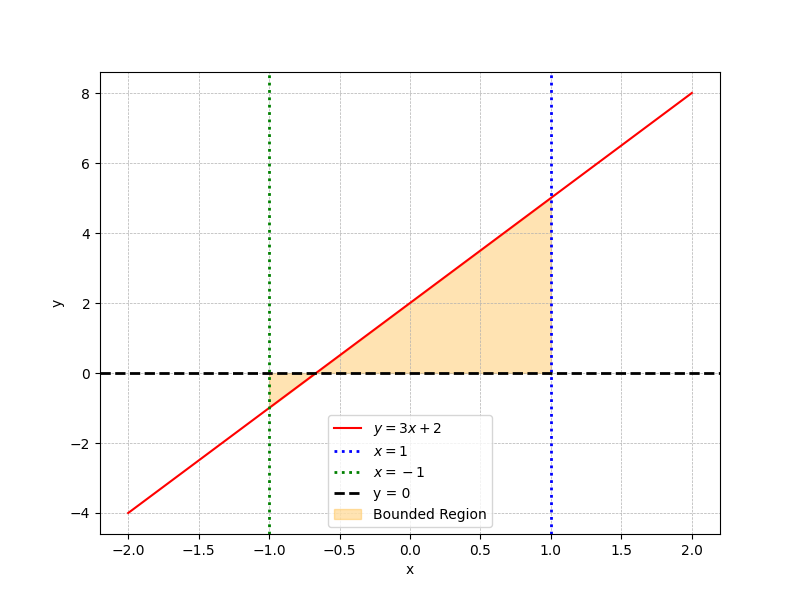
\includegraphics[width=\columnwidth]{figs/fig.png}
 \end{figure}
\end{frame}
\end{document}
